\section{Exception handling in five stage pipelines}

Exceptions may arise at various stages within the pipeline. 
However, the recommended approach for interrupt handling is to minimize pipeline interruption as much as possible.
\begin{figure}[H]
    \centering
    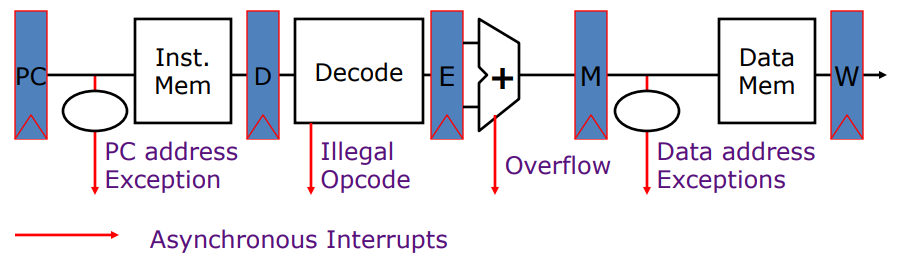
\includegraphics[width=0.75\linewidth]{images/5s.png}
    \caption{Exception origins}
\end{figure}
To address this, instructions in the pipeline can be tagged to indicate whether they cause exceptions or not. 
This tagging process waits until the memory stage concludes before flagging an exception. 
Interrupts are then represented as No-Operation (NOP) placeholders inserted into the pipeline instead of regular instructions.

In cases where a NOP is flushed, it is assumed that the interrupt condition persists.
However, managing interrupt conditions becomes complex due to requirements such as supervisor mode switching and saving one or more program counters (PCs).

Additionally, optimizing instruction fetch to start fetching instructions from the interrupt vector may be challenging due to these complexities.
\begin{figure}[H]
    \centering
    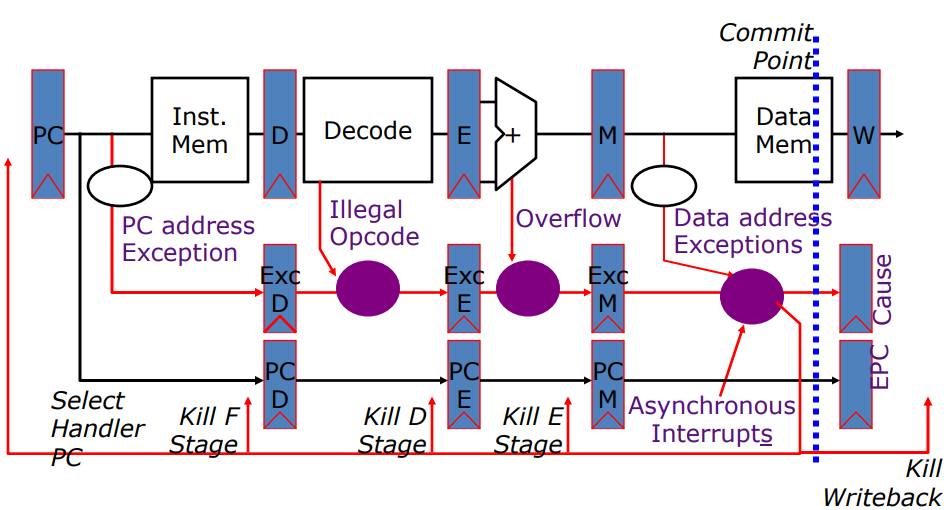
\includegraphics[width=0.75\linewidth]{images/5s2.png}
    \caption{Exception handling}
\end{figure}
Maintain exception flags within the pipeline until reaching the commit point (M stage). 
Exceptions occurring in earlier pipeline stages take precedence over later ones for a particular instruction. 
External interrupts are injected at the commit point, overriding any other exceptions present.

If an exception occurs at the commit point, cause and EPC registers are updated, all pipeline stages are terminated, and the handler PC is injected into the fetch stage.

Jim Smith's paper explores various techniques for achieving precise interrupts, including in-order instruction completion, reorder buffer, and history buffer methodologies.

\subsection{Remarks}
The possible methods to anticipate the exceptions are: 
\begin{itemize}
    \item \textit{Prediction mechanism}: due to the infrequent occurrence of exceptions, a straightforward prediction of no exceptions yields high accuracy.
    \item \textit{Verification of prediction mechanism}: exceptions are identified at the conclusion of the instruction execution pipeline, utilizing specialized hardware tailored for different exception types.
    \item \textit{Recovery mechanism}:architectural state is exclusively written at the commit point, enabling the discarding of partially executed instructions after an exception.
        Following the exception, the pipeline is flushed, and the exception handler is initiated.
    \item \textit{Bypassing}: bypassing facilitates the utilization of uncommitted instruction outcomes by subsequent instructions.
\end{itemize}